\documentclass[11pt,a4paper]{article}
\usepackage[utf8]{inputenc}
\usepackage[spanish]{babel}	%Idioma
\usepackage{amsmath}
\usepackage{amsfonts}
\usepackage{amssymb}
\usepackage{graphicx} 	%Añadir imágenes
\usepackage{geometry}	%Ajustar márgenes
\usepackage[export]{adjustbox}[2011/08/13]
\usepackage{float}
\restylefloat{table}
\usepackage[hidelinks]{hyperref}
\usepackage{titling}
\graphicspath{{/home/nazaret/Escritorio/LaTEX}}
%\usepackage{minted}
\usepackage{multirow}
\usepackage{caption}
\usepackage{multicol}
\usepackage[shortlabels]{enumitem}
\usepackage{array}
\selectlanguage{spanish}

%Opciones de encabezado y pie de página:
\usepackage{fancyhdr}
\pagestyle{fancy}
\lhead{Nazaret Román Guerrero}
\rhead{Redes Multiservicio}
\lfoot{Grado en Ingeniería Informática}
\cfoot{}
\rfoot{\thepage}
\renewcommand{\headrulewidth}{0.4pt}
\renewcommand{\footrulewidth}{0.4pt}

%Opciones de fuente:
\usepackage[utf8]{inputenc}
\usepackage[default]{sourcesanspro}
\usepackage{sourcecodepro}
\usepackage[T1]{fontenc}

\setlength{\parindent}{15pt}
\setlength{\headheight}{15pt}
\setlength{\voffset}{10mm}

% Custom colors
\usepackage{color}
\definecolor{deepblue}{rgb}{0,0,0.5}
\definecolor{deepred}{rgb}{0.6,0,0}
\definecolor{deepgreen}{rgb}{0,0.5,0}

\usepackage{xcolor}
\usepackage{listings}
\lstset{basicstyle=\ttfamily, basicstyle=\footnotesize,
  showstringspaces=false,
  commentstyle=\color{red},
  keywordstyle=\color{blue}
}

\begin{document}
\begin{titlepage}

\begin{minipage}{\textwidth}

\centering

\includegraphics[width=0.6\textwidth]{img/logo.png}\\

\textsc{\Large Redes Multiservicio\\[0.2cm]}
\textsc{GRADO EN INGENIERÍA INFORMÁTICA}\\[1cm]

{\Huge\bfseries Análisis de \textit{streaming}: \textit{Netflix}\\}
\noindent\rule[-1ex]{\textwidth}{3pt}\\[3.5ex]
{\large\bfseries Tarea 4}
\end{minipage}

\vspace{1cm}
\begin{minipage}{\textwidth}
\centering

\textbf{Autora}\\ {Nazaret Román Guerrero}\\[2.5ex]

\includegraphics[width=0.35\textwidth]{img/etsiit.jpeg}\\[0.1cm]
\vspace{0.5cm}
\textsc{Escuela Técnica Superior de Ingenierías Informática y de Telecomunicación}\\
\vspace{0.5cm}
\textsc{Curso 2018-2019}
\end{minipage}
\end{titlepage}

\pagenumbering{gobble}
\pagenumbering{arabic}

\newpage

\section*{\textit{Netflix}: cómo funciona}

\textit{Netflix} es una aplicación de streaming que se utiliza para ver series y películas. A diferencia de \textit{spotify} donde tienes dos opciones de uso (gratis o pagando), en \textit{netflix} es \textbf{obligatorio} pagar una subscripción, ya sea por meses o de forma anual. Hay distintos tipos de tarifas y planes dependiendo de si eres estudiante, si es para compartir con tu familia...\\

Al igual que con \textit{spotify} puede funcionar a través de una aplicación de escritorio, con el navegador, aplicaciones para dispositivos \textit{android} o \textit{IOS}... Para cambiar de método con respecto al trabajo de \textit{spotify}, voy a utilizar el navegador.\\

He cogido un total de 2317 paquetes, pero no todos son paquetes con datos de vídeo o audio. Filtrando con el filtro \color{deepgreen}\texttt{ip.src==212.230.193.37 \&\& ssl.app\_data}\color{black}, salen un total de 1801 paquetes de datos.

%filtro: ip.src==212.230.193.37 && ssl.app_data

\subsection*{Datos relacionados con los paquetes enviados}

\textit{Netflix} envía distintos tipos de paquetes dependiendo de la acción que se lleve a cabo: si se pausa el vídeo, si se reactiva, si se entra en modo de pantalla completa, si se requieren más paquetes para cargar el vídeo o el audio...

\begin{itemize}
	\item \textbf{Tamaño de los paquetes}: hablando de los paquetes que contienen puramente información sobre el vídeo o el audio (paquetes cuyo contenido es \textit{Application data}), el tamaño de éstos varía. Para sacar un tamaño medio vamos a filtrar primero la captura de wireshark con el filtro: \color{deepgreen}\texttt{ip.src==212.230.193.37 \&\& ssl.app\_data}\color{black}.
	
	Una vez que está filtrado, vamos a sacar una media con el tamaño de los paquetes. Para ello tomamos el campo \texttt{length} y le restamos el tamaño de la cabecera, de 40 bytes.
	
	Como ejemplo vamos a mostrar el siguiente fragmento de paquetes enviados:
	
	\begin{figure}[H]
		\centering
		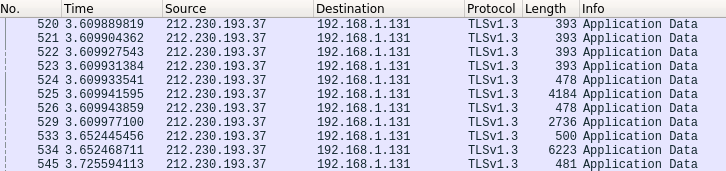
\includegraphics[scale=0.5]{img/frag-netflix-size.png}
	\end{figure}
\end{itemize}

	Al calcular la media de los paquetes sale un tamaño de 393,5 bytes por paquete enviado. A pesar de haber algunos picos como se pueden ver en la imagen anterior, la distribución de tamaños es bastante uniforme entre 350 y 450 aproximadamente, a diferencia de \textit{spotify}, donde había mucha diferencia de tamaños entre paquetes.\\
	
	El tamaño también depende de la calidad de visualización. Puesto que en el navegador el límite son 720p, los paquetes no son tan grandes como lo serían en el caso de que la reproducción fuese en HD.


\subsection*{Datos relacionados con el envío de paquetes}

\begin{itemize}
	\item \textbf{Protocolo de transporte:} los paquetes son enviados a través de TCP. La información va envuelta en el protocolo SSL para proteger y encriptar los datos enviados, con la versión TLSv1.3. En este caso no he encontrado ningún patrón en el envío como en \textit{spotify}, donde se cambiaba la versión del cifrado en mitad del envío.
	
	\item \textbf{Puerto:} el puerto que recibe los paquetes es el 443. La información disponible en la página de soporte de \textit{netflix} es muy limitada, tanto que ni siquiera indica si llevan a cabo \textit{tunneling}. La compañía es muy recelosa sobre sus datos y exponen los mínimos posibles en la web, por lo que lo único que podemos saber es el puerto fuente gracias a la captura de \textit{wireshark}; en la siguiente imagen se puede ver:
	
	\begin{figure}[H]
		\centering
		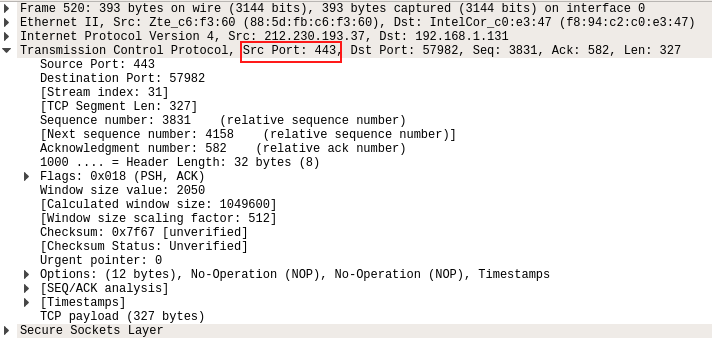
\includegraphics[scale=0.5]{img/puerto-netflix.png}
	\end{figure}
	
	\item \textbf{Frecuencia de envío}: los paquetes que se envían según el cliente necesite o pueda soportar. Es decir, si el cliente no tiene restricciones y una buena conexión, \textit{netflix} envía paquetes para cargar el vídeo y el audio de manera rápida para que no se produzcan cortes en la visualización. Vamos a calcular la frecuencia media de envío en la captura de \textit{wireshark} que he cogido.
	
	La frecuencia calculada es 0.011872 segundos, es decir, cuando pasa ese tiempo aproximadamente se envía un nuevo paquete de datos (de audio o de vídeo). No se puede diferenciar entre ambos ya que no hay información visible sobre el contenido de los paquetes que se están transmitiendo, y puesto que todos tienen un tamaño similar tampoco podemos saber si es vídeo o audio por el tamaño.
	
	\item \textbf{Bitrate medio}: ahora vamos a calcular la tasa media. Para ello, debemos tomar los bytes enviados en cada paquete y dividirlo entre el tiempo que ha tardado en ser enviado. Una vez tenemos estos datos, solo debemos hacer la media.
	
	La media es un envío de 4.349 Mbps. Si lo comparamos con la tasa media de envío de \textit{spotify}, vemos que es mucho menor, casi 3 Mb menos por segundo.
	
	Es fácil pensar que el tráfico que genera una aplicación de streaming de vídeo es mucho más pesado y lento que el tráfico generado por una aplicación de streaming de solo audio.
	
	\item \textbf{Bitrate pico}: finalmente, para calcular el bitrate pico, vamos a buscar el paquete que se ha enviado con una mayor tasa, es decir, donde el cociente entre los bytes enviados y el tiempo de envío es el mayor. En este caso, el bitrate pico es de 5.274 Mbps, lo que no supone una subida excesiva con respecto a la media, no aumenta ni siquiera 1 Mbps más.
\end{itemize}

\end{document}